\documentclass{article}
\usepackage{mathrsfs}
\usepackage{amsmath,amssymb,amsthm}
\usepackage{enumitem}
\usepackage{tikz}
\usetikzlibrary{shapes.geometric, arrows.meta, positioning}

\theoremstyle{plain}
\newtheorem{theorem}{Theorem}[section]
\newtheorem{lemma}[theorem]{Lemma}
\newtheorem{proposition}[theorem]{Proposition}
\newtheorem{notation}{Notation}
\newtheorem{corollary}[theorem]{Corollary}
\newtheorem{definition}[theorem]{Definition}
\newtheorem{example}[theorem]{Example}
\newtheorem{remark}[theorem]{Remark}

\theoremstyle{remark}
\newtheorem*{acknowledgment}{Acknowledgment}

\title{Comprehension Categories and the Semantics of Type Dependency}
\author{Bart Jacobs \\ Department of Mathematics, University of Utrecht \\ P.O. Box 80.010, 3508 TA Utrecht, The Netherlands \\ Email: bjacobs@math.ruu.nl}
\date{Received June 1990 \\ Revised August 1991}

\begin{document}

\maketitle

\begin{abstract}
A comprehension category is defined as a functor $\mathscr{P}: \mathbf{E} \to \mathbf{B}^{\to}$ satisfying (a) $\operatorname{cod} \circ \mathscr{P}$ is a fibration, and (b) $f$ is cartesian in $\mathbf{E}$ implies that $\mathscr{P} f$ is a pullback in $\mathbf{B}$. This notion captures many structures used to describe type dependency, such as display-map categories, categories with attributes, D-categories, and comprehensive fibrations. It also encompasses comprehension as occurring in topos theory and Lawvere's hyperdoctrines. This paper introduces comprehension categories, defining a closed comprehension category as one with dependent products and sums. Examples are provided, with further details in Jacobs (1991) and applications in Jacobs et al. (1991).
\end{abstract}

\tableofcontents

\newpage
\section{Introduction}

The term ``type dependency'' refers to the ability in a calculus of types and terms to have types that depend on term variables, as studied by de Bruijn \cite{deBruijn1970} and Martin-L\"of \cite{MartinLof1984}. In computer science, type dependency is useful, e.g., to define $\operatorname{List}(n)$ as the type of lists of length $n$. Unlike polymorphic calculi, languages with type dependency blur the distinction between compile time and run time. This paper focuses on the categorical semantics of type dependency, referring to \cite{MartinLof1984, Troelstra1986} for syntactic details.

A key challenge in categorical semantics is modeling contexts, which cannot be simple cartesian products due to dependencies among types. Specifically, we address context extension, i.e., the transition from $\Gamma \vdash \sigma : \text{Type}$ to the extended context $\Gamma, x : \sigma$. In categorical logic, statements $\Gamma \vdash \sigma : \text{Type}$ are viewed as objects fibred over contexts $\Gamma$, requiring a fibration $p : \mathbf{E} \to \mathbf{B}$. Context extension is modeled by a functor $\mathscr{P}_0 : \mathbf{E} \to \mathbf{B}$, equipped with a natural transformation $\mathscr{P}_0 \to p$, where components are projections $\Gamma, x : \sigma \to \Gamma$. This structure corresponds to a functor $\mathbf{E} \to \mathbf{B}^{\to}$, where $\mathbf{B}^{\to}$ is the arrow category of $\mathbf{B}$. By requiring projections to be stable under substitution (see Lemma \ref{lem:4.4}), we define comprehension categories.

Various categorical structures for type dependency have been proposed over the past 15 years \cite{Cartmell1978, Seely1984, Taylor1986, Lamarche1988, HylandPitts1989, Moggi1991, Pavlovic1990}. Despite differences, context extension is a common feature. Comprehension categories provide a minimal, clean categorical framework, further developed in \cite{Jacobs1991, JacobsMoggiStreicher1991}, where they serve as building blocks for arbitrary type systems.

Comprehension categories involve a weak form of comprehension, described by disjoint unions (see after Lemma \ref{lem:4.4}), handling context extension in $\Gamma, x : \sigma$. Other notions of comprehension (Pavlović, Ehrhard, Lawvere) fit within this framework.

We view category theory as an assembly language, requiring detailed handling of substitution and isomorphisms, while type theory acts as a higher-level language for parts of category theory, with interpretation akin to compilation. Category theory thus provides a variable-free formalism for logic and type theory, central to categorical abstract machines \cite{Curien1986, Curien1989}.

The paper begins with fibred category theory (Sections \ref{sec:fibrations} and \ref{sec:category-theory-basis}), covering standard material from Grothendieck and Bénabou. Fibrations are the backbone of comprehension categories, and fibred adjunctions ensure substitution properties like $(\lambda x : \sigma . P)[x := M] = \lambda x : \sigma[x := M] . (P[x := M])$. Section \ref{sec:comprehension-categories} introduces comprehension categories, showing how examples fit, while Section \ref{sec:quantification} addresses quantification.

\newpage
\section{Fibrations}
\label{sec:fibrations}

We present basic facts about fibrations; see \cite{Benabou1985, Giraud1971, Gray1966, Grothendieck1971} for details. Parentheses are often omitted for readability.

\begin{definition}
\label{def:2.1}
Let $p : \mathbf{E} \to \mathbf{B}$ be a functor.
\begin{enumerate}
    \item[(i)] A morphism $f : D \to E$ in $\mathbf{E}$ is \emph{cartesian} over $u : A \to B$ in $\mathbf{B}$ if:
        \begin{itemize}
            \item[(a)] $p f = u$,
            \item[(b)] for every $f' : D' \to E$ with $p f' = u$, there is a unique $\phi : D' \to D$ with $p \phi = \text{id}_A$ and $f' = f \circ \phi$.
        \end{itemize}
    \item[(ii)] Dually, $g : D \to E$ is \emph{cocartesian} over $u$ if $g$ in $\mathbf{E}^{\text{op}}$ is cartesian over $u$ in $\mathbf{B}^{\text{op}}$, i.e.:
        \begin{itemize}
            \item[(a)] $p g = u$,
            \item[(b)] for every $g' : D \to E'$ with $p g' = u$, there is a unique $\psi : E \to E'$ with $p \psi = \text{id}_B$ and $g' = \psi \circ g$.
        \end{itemize}
\end{enumerate}
This is shown in Figure \ref{fig:cartesian-cocartesian}. A cartesian $f$ is a \emph{terminal lifting}, and a cocartesian $g$ is an \emph{initial lifting} of $u$.
\begin{figure}[h]
    \centering
    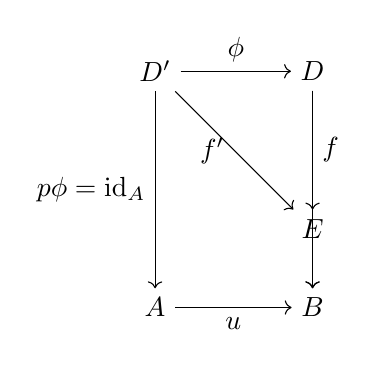
\begin{tikzpicture}
        \node (D') at (0,2) {$D'$};
        \node (D) at (2,2) {$D$};
        \node (E) at (2,0) {$E$};
        \node (A) at (0,-1) {$A$};
        \node (B) at (2,-1) {$B$};
        \draw[->] (D') to node[above] {$\phi$} (D);
        \draw[->] (D) to node[right] {$f$} (E);
        \draw[->] (D') to node[left] {$f'$} (E);
        \draw[->] (A) to node[below] {$u$} (B);
        \draw[->] (D') to node[left] {$p \phi = \text{id}_A$} (A);
        \draw[->] (D) to (B);
        \draw[->] (E) to (B);
    \end{tikzpicture}
    \caption{Cartesian morphism diagram.}
    \label{fig:cartesian-cocartesian}
\end{figure}
\begin{enumerate}
    \item[(iii)] The functor $p : \mathbf{E} \to \mathbf{B}$ is a \emph{fibration} if:
        \begin{itemize}
            \item[(a)] for every $E \in \mathbf{E}$ and $u : A \to p E$ in $\mathbf{B}$, there is a cartesian $f : D \to E$ over $u$ in $\mathbf{E}$;
            \item[(b)] the composition of two cartesian morphisms is cartesian.
        \end{itemize}
        $\mathbf{B}$ is the \emph{base category}, and $\mathbf{E}$ is the \emph{total category}. Dually, $p$ is a \emph{cofibration} if $p^{\text{op}} : \mathbf{E}^{\text{op}} \to \mathbf{B}^{\text{op}}$ is a fibration. A \emph{bifibration} is both a fibration and a cofibration.
\end{enumerate}
\end{definition}

The arrow category $\mathbf{B}^{\to}$ has arrows of $\mathbf{B}$ as objects and commuting squares as morphisms. The functor $\operatorname{dom} : \mathbf{B}^{\to} \to \mathbf{B}$ is a fibration. If $\mathbf{B}$ has pullbacks, $\operatorname{cod} : \mathbf{B}^{\to} \to \mathbf{B}$ is a bifibration, with cartesian morphisms as pullback squares. Modules over rings provide another bifibration example \cite{Gray1966}.

Cartesian (cocartesian) morphisms are denoted $\bar{u}(E) : u^*(E) \to E$ ($\underline{u}(D) : D \to u_*(D)$), unique up to isomorphism. A morphism $f : D \to E$ is \emph{strong cartesian} over $u : A \to B$ if $p f = u$ and for any $f' : D' \to E$ with $p f' = u \circ v$, there is a unique $\phi : D' \to D$ with $p \phi = v$ and $f' = f \circ \phi$. For fibrations, cartesian and strong cartesian morphisms coincide.

\begin{definition}
\label{def:2.2}
Let $p : \mathbf{E} \to \mathbf{B}$ be a functor. For $B \in \mathbf{B}$, the \emph{fibre} $\mathbf{E}_B$ is the category with objects $E \in \mathbf{E}$ such that $p E = B$ and arrows $f$ in $\mathbf{E}$ with $p f = \text{id}_B$ (vertical morphisms).
\end{definition}

For $E, D \in \mathbf{E}$ and $u : p E \to p D$, define $\mathbf{E}_u(D, E) = \{ f \in \mathbf{E}(D, E) \mid p f = u \}$. If $p$ is a fibration, $\mathbf{E}_u(D, E) \cong \mathbf{E}_{p D}(D, u^*(E))$; if a cofibration, $\mathbf{E}_u(D, E) \cong \mathbf{E}_{p E}(u_*(D), E)$.

For a fibration $p$ and $u : A \to B$, define $u^*(f) : u^*(E) \to u^*(D)$ in $\mathbf{E}_A$ for $f : E \to D$ in $\mathbf{E}_B$ using the cartesian morphism $\bar{u}(D) : u^*(D) \to D$ (see Figure \ref{fig:reindexing}).
\begin{figure}[h]
    \centering
    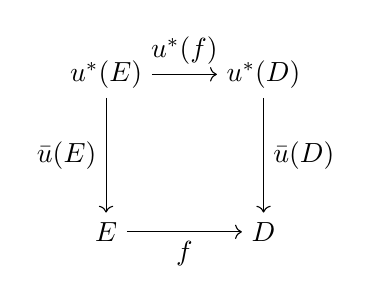
\begin{tikzpicture}
        \node (uE) at (0,2) {$u^*(E)$};
        \node (uD) at (2,2) {$u^*(D)$};
        \node (E) at (0,0) {$E$};
        \node (D) at (2,0) {$D$};
        \draw[->] (uE) to node[above] {$u^*(f)$} (uD);
        \draw[->] (uE) to node[left] {$\bar{u}(E)$} (E);
        \draw[->] (uD) to node[right] {$\bar{u}(D)$} (D);
        \draw[->] (E) to node[below] {$f$} (D);
    \end{tikzpicture}
    \caption{Reindexing functor diagram.}
    \label{fig:reindexing}
\end{figure}
This yields a pullback in $\mathbf{E}$, and $u^* : \mathbf{E}_B \to \mathbf{E}_A$ is the \emph{reindexing functor}. A \emph{cleavage} is a collection $\{ u^*, \bar{u} \}$ satisfying certain natural isomorphisms. A fibration is \emph{split} if $\bar{v} \circ \bar{u}(E) = \bar{v}(E) \circ \bar{u}(v^*(E))$ and $\bar{\text{id}}(E) = \text{id}_E$.

The Grothendieck construction yields a split fibration from a functor $\Psi : \mathbf{B}^{\text{op}} \to \text{Cat}$, with objects $(A, X)$, $X \in \Psi A$, and morphisms $(u, f) : (A, X) \to (B, Y)$, where $u : A \to B$ and $f : X \to \Psi(u)(Y)$.

\begin{proposition}
\label{prop:2.3}
Let $p : \mathbf{E} \to \mathbf{B}$ be a fibration.
\begin{enumerate}
    \item[(i)] $p$ is a bifibration if and only if every $u^*$ has a left adjoint $\Sigma_u$.
    \item[(ii)] If $r : \mathbf{B} \to \mathbf{A}$ is a fibration, then $r p : \mathbf{E} \to \mathbf{A}$ is a fibration.
\end{enumerate}
\end{proposition}

\begin{definition}
\label{def:2.4}
\begin{enumerate}
    \item[(i)] For fibrations $p : \mathbf{E} \to \mathbf{B}$ and $q : \mathbf{D} \to \mathbf{B}$, a functor $H : \mathbf{E} \to \mathbf{D}$ is \emph{cartesian} if $q \circ H = p$ and $H$ preserves cartesian morphisms. This defines a category $\text{Fib}(\mathbf{B})$. More generally, $\text{Fib}$ has morphisms $(H, K) : (p : \mathbf{E} \to \mathbf{B}) \to (q : \mathbf{D} \to \mathbf{A})$ where $q \circ H = K \circ p$ and $H$ preserves cartesian morphisms.
    \item[(ii)] $\text{Fib}(\mathbf{B})$ and $\text{Fib}$ are 2-categories with 2-cells $\sigma : H \to H'$ (in $\text{Fib}(\mathbf{B})$) or $(\sigma, \tau) : (H, K) \to (H', K')$ (in $\text{Fib}$) as natural transformations with vertical components.
\end{enumerate}
\end{definition}

\begin{lemma}
\label{lem:2.5}
Let $p : \mathbf{E} \to \mathbf{B}$, $q : \mathbf{D} \to \mathbf{B}$ be fibrations, and $F : p \to q$ a cartesian functor.
\begin{enumerate}
    \item[(i)] $F$ restricts to $\left.F\right|_A : \mathbf{E}_A \to \mathbf{D}_A$. $F$ is full (faithful) if and only if every $\left.F\right|_A$ is full (faithful).
    \item[(ii)] If $F$ is full and faithful, $f$ is $p$-cartesian if and only if $F f$ is $q$-cartesian.
\end{enumerate}
\end{lemma}

\begin{proposition}
\label{prop:2.6}
\begin{enumerate}
    \item[(i)] The pullback in $\text{Cat}$ of a fibration $p : \mathbf{E} \to \mathbf{B}$ and $K : \mathbf{A} \to \mathbf{B}$ yields a fibration $K^*(p) : \mathbf{A} \underset{K, p}{\times} \mathbf{E} \to \mathbf{A}$ and a morphism $K^*(p) \to p$.
    \item[(ii)] The functor $\text{Fib} \to \text{Cat}$, mapping a fibration to its base, is a fibration with fibres $\text{Fib}(\mathbf{B})$.
    \item[(iii)] $\text{Fib}(\mathbf{B})$ has finite products, preserved under change-of-base.
\end{enumerate}
\end{proposition}

\newpage
\section{Category Theory over a Basis}
\label{sec:category-theory-basis}

Since $\text{Fib}(\mathbf{B})$ is a 2-category, we define fibred adjunctions.

\begin{definition}
\label{def:3.1}
For fibrations $p : \mathbf{E} \to \mathbf{B}$, $q : \mathbf{D} \to \mathbf{B}$, and cartesian functors $F : p \to q$, $G : q \to p$, $F$ is a \emph{fibred left adjoint} of $G$ if $F \dashv G$ with a vertical unit $\eta$.
\end{definition}

\begin{definition}
\label{def:3.2}
For adjunctions $F \dashv G$ ($F : \mathbf{E} \to \mathbf{D}$) and $F' \dashv G'$ ($F' : \mathbf{E}' \to \mathbf{D}'$), a \emph{pseudo map} from $F \dashv G$ to $F' \dashv G'$ is a quadruple $(K, L, \varphi, \psi)$ with functors $K : \mathbf{E} \to \mathbf{E}'$, $L : \mathbf{D} \to \mathbf{D}'$, and natural isomorphisms $\varphi : F' K \to L F$, $\psi : G' L \to K G$, preserving units and counits (see Figure \ref{fig:pseudo-map}).
\begin{figure}[h]
    \centering
    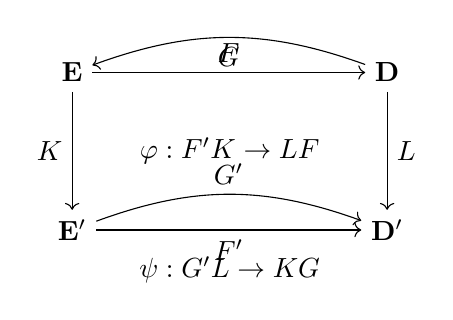
\begin{tikzpicture}
        \node (E) at (0,2) {$\mathbf{E}$};
        \node (D) at (4,2) {$\mathbf{D}$};
        \node (E') at (0,0) {$\mathbf{E}'$};
        \node (D') at (4,0) {$\mathbf{D}'$};
        \draw[->] (E) to node[above] {$F$} (D);
        \draw[->] (E') to node[below] {$F'$} (D');
        \draw[->] (E) to node[left] {$K$} (E');
        \draw[->] (D) to node[right] {$L$} (D');
        \draw[->, bend left=20] (E') to node[above] {$G'$} (D');
        \draw[->, bend right=20] (D) to node[below] {$G$} (E);
        \node at (2,1) {$\varphi : F' K \to L F$};
        \node at (2,-0.5) {$\psi : G' L \to K G$};
    \end{tikzpicture}
    \caption{Pseudo map of adjunctions.}
    \label{fig:pseudo-map}
\end{figure}
\end{definition}

\begin{lemma}
\label{lem:3.3}
In Definition \ref{def:3.2}, $\varphi$ and $\psi$ determine each other: an isomorphism $F' K \cong L F$ induces a pseudo map if and only if the canonical transformation $K G \to G' L$ is an isomorphism, and similarly for $G' L \cong K G$.
\end{lemma}

\begin{proposition}
\label{prop:3.4}
For a cartesian functor $F : p \to q$ in $\text{Fib}(\mathbf{B})$ with right adjoints $G_A$ for each $\left.F\right|_A$, the following are equivalent:
\begin{enumerate}
    \item[(i)] $F$ has a fibred right adjoint $G$ underlying $\{ G_A \}$.
    \item[(ii)] For every $u : A \to B$, reindexing functors $u^{*p}$, $u^{*q}$ determine a pseudo map $\left.F\right|_B \dashv G_B \to \left.F\right|_A \dashv G_A$.
    \item[(iii)] For every $u : A \to B$, the canonical transformation $u^{*p} G_B \to G_A u^{*q}$ is an isomorphism.
\end{enumerate}
\end{proposition}

\begin{definition}
\label{def:3.5}
A fibration $p : \mathbf{E} \to \mathbf{B}$ \emph{admits a terminal object} if the unique morphism $p \to \text{terminal}$ in $\text{Fib}(\mathbf{B})$ has a fibred right adjoint. Thus, each fibre $\mathbf{E}_A$ has a terminal object $1 A$, and $u^*(1 B) \to 1 A$ is an isomorphism for $u : A \to B$.
\end{definition}

\begin{definition}
\label{def:3.6}
A fibration $p : \mathbf{E} \to \mathbf{B}$ \emph{admits cartesian products} if the morphism $\Delta : p \to p \times p$ in $\text{Fib}(\mathbf{B})$ has a fibred right adjoint. Thus, each fibre $\mathbf{E}_A$ has products $(-) \times_A (-)$, and the canonical map $u^*(E \times_B D) \to u^*(E) \times_A u^*(D)$ is an isomorphism.
\end{definition}

\begin{definition}
\label{def:3.7}
A fibration $p : \mathbf{E} \to \mathbf{B}$ \emph{admits equalizers} if the morphism $\Delta : p \to p^{2+}$ in $\text{Fib}(\mathbf{B})$ has a fibred right adjoint, where $p^{2+}$ is defined via change-of-base.
\end{definition}

\begin{lemma}
\label{lem:3.8}
For a bifunctor $F : \mathbf{A} \times \mathbf{P} \to \mathbf{B}$, the following are equivalent:
\begin{enumerate}
    \item[(i)] For each $p \in \mathbf{P}$, $F(-, p)$ has a right adjoint $G(-, p)$.
    \item[(ii)] For every groupoid subcategory $|\mathbf{P}|$ of $\mathbf{P}$ with $\text{Obj}|\mathbf{P}| = \text{Obj} \mathbf{P}$, the functor $\tilde{F} : \mathbf{A} \times |\mathbf{P}| \to \mathbf{B} \times |\mathbf{P}|$ has a right adjoint $\tilde{G}$.
    \item[(iii)] There exists such a groupoid $|\mathbf{P}|$ satisfying (ii).
\end{enumerate}
\end{lemma}

\begin{definition}
\label{def:3.9}
A fibration $p : \mathbf{E} \to \mathbf{B}$ with cartesian products \emph{admits exponents} if the functor $\widetilde{\text{prod}} : p \times |p| \to p \times |p|$ in $\text{Fib}(\mathbf{B})$ has a fibred right adjoint.
\end{definition}

\begin{definition}
\label{def:3.10}
Let $p : \mathbf{E} \to \mathbf{B}$ be a fibration, where $\mathbf{B}$ has pullbacks.
\begin{enumerate}
    \item[(i)] $p$ \emph{has sums} if every $u^*$ has a left adjoint $\Sigma_u$, and the Beck-Chevalley condition holds: for a pullback in $\mathbf{B}$, $\Sigma_u s^* \to r^* \Sigma_v$ is an isomorphism.
    \item[(ii)] $p$ \emph{has products} if $u^* \dashv \Pi_u$ and $r^* \Pi_v \cong \Pi_u s^*$ canonically.
\end{enumerate}
\end{definition}

For a category $\mathbf{B}$ with finite limits, $\operatorname{cod} : \mathbf{B}^{\to} \to \mathbf{B}$ has fibred finite limits and sums. $\mathbf{B}$ is a locally cartesian-closed category (LCCC) if $\operatorname{cod} : \mathbf{B}^{\to} \to \mathbf{B}$ is a fibred CCC.

\section{Comprehension Categories}
\label{sec:comprehension-categories}

\begin{definition}
\label{def:4.1}
A \emph{comprehension category} is a functor $\mathscr{P} : \mathbf{E} \to \mathbf{B}^{\to}$ satisfying:
\begin{enumerate}
    \item[(i)] $\operatorname{cod} \circ \mathscr{P} : \mathbf{E} \to \mathbf{B}$ is a fibration.
    \item[(ii)] If $f$ is cartesian in $\mathbf{E}$, then $\mathscr{P} f$ is a pullback in $\mathbf{B}$.
\end{enumerate}
It is \emph{full} if $\mathscr{P}$ is full and faithful, and \emph{cloven} or \emph{split} if the fibration is cloven or split.
\end{definition}

\begin{notation}
\label{not:4.2}
For a comprehension category $\mathscr{P} : \mathbf{E} \to \mathbf{B}^{\to}$, write $p = \operatorname{cod} \circ \mathscr{P}$, $\mathscr{P}_0 = \operatorname{dom} \circ \mathscr{P}$. The object part of $\mathscr{P}$ is a natural transformation $\mathscr{P} : \mathscr{P}_0 \to p$. For $E \in \mathbf{E}$, $\mathscr{P} E$ are \emph{projections}, $\mathscr{P} E^*$ are \emph{weakening functors}, and $|E| = \{ u : p E \to \mathscr{P}_0 E \mid \mathscr{P} E \circ u = \text{id} \}$ are \emph{terms} of type $E$.
\end{notation}

\begin{example}
\label{ex:4.3}
(Term model) For a calculus with type dependency \cite{MartinLof1984, Troelstra1986}, define a full comprehension category $\mathscr{P} : \mathbf{E} \to \mathbf{B}^{\to}$. Objects of $\mathbf{B}$ are equivalence classes $[\Gamma]$ of contexts. Morphisms $[\Gamma] \to [\Delta]$, with $\Delta \equiv y_1 : \tau_1, \ldots, y_n : \tau_n$, are $n$-tuples $\langle [M_1], \ldots, [M_n] \rangle$ where $\Gamma \vdash M_i : \tau_i[x_1 := M_1, \ldots, x_{i-1} := M_{i-1}]$. Objects of $\mathbf{E}$ are $[\Gamma \vdash \sigma : \text{Type}]$, and arrows are pairs $([\bar{M}], [N])$ with $[\bar{M}] : [\Gamma] \to [\Delta]$ and $\Gamma, x : \sigma \vdash N : \tau[\hat{y} := \bar{M}]$. Then $\mathscr{P} : [\Gamma \vdash \sigma : \text{Type}] \mapsto ([\Gamma, x : \sigma] \to [\Gamma])$.
\end{example}

\begin{lemma}
\label{lem:4.4}
For a comprehension category $\mathscr{P} : \mathbf{E} \to \mathbf{B}^{\to}$, for every $E \in \mathbf{E}$ and $u : A \to p E$, there is a pullback as in Figure \ref{fig:pullback-4.4}. Thus, a pullback functor $\mathscr{P} E^* : \mathbf{B}/p E \to \mathbf{B}/\mathscr{P}_0 E$ is defined by $u \mapsto \mathscr{P}_0 \bar{u}(E)$.
\begin{figure}[h]
    \centering
    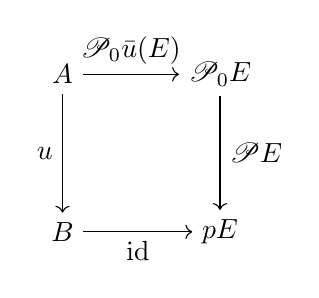
\begin{tikzpicture}
        \node (A) at (0,2) {$A$};
        \node (P0E) at (2,2) {$\mathscr{P}_0 E$};
        \node (pE) at (2,0) {$p E$};
        \node (B) at (0,0) {$B$};
        \draw[->] (A) to node[above] {$\mathscr{P}_0 \bar{u}(E)$} (P0E);
        \draw[->] (A) to node[left] {$u$} (B);
        \draw[->] (P0E) to node[right] {$\mathscr{P} E$} (pE);
        \draw[->] (B) to node[below] {$\text{id}$} (pE);
    \end{tikzpicture}
    \caption{Pullback for Lemma \ref{lem:4.4}.}
    \label{fig:pullback-4.4}
\end{figure}
\end{lemma}

For $E \in \mathbf{E}$ above $B \in \mathbf{B}$ and $u : A \to B$, there is an isomorphism $\mathbf{B}/\mathbf{B}(u, \mathscr{P} E) \cong |u^*(E)|$, encoding a disjoint union.

\begin{example}
\label{ex:4.5}
(Display-map categories) If $\mathbf{B}$ has pullbacks, the identity $\mathbf{B}^{\to} \to \mathbf{B}^{\to}$ is a full comprehension category. For a category $\mathbf{B}$ with a collection $\mathscr{D}$ of display maps closed under pullbacks \cite{Taylor1986, HylandPitts1989, Lamarche1988}, the inclusion $\mathbf{B}^{\to}(\mathscr{D}) \subset \mathbf{B}^{\to}$ is a full comprehension category.
\end{example}

\begin{example}
\label{ex:4.6}
(Full internal subcategories) For an LCCC $\mathbf{B}$ and morphism $\tau$, the fibration $\Sigma(\tau) \to \mathbf{B}$ has a full and faithful cartesian functor $\Sigma(\tau) \to \mathbf{B}^{\to}$, forming a full comprehension category \cite{Pitts1987, Johnstone1977}.
\end{example}

\begin{example}
\label{ex:4.7}
(Topos comprehension) For a topos $\mathbf{B}$ with subobject classifier $\top : t \to \Omega$, the functor $\mathbf{B}/\Omega \to \mathbf{B}^{\to}$ mapping $\varphi : A \to \Omega$ to its extension is a comprehension category, full and faithful on $\operatorname{Cart}(\mathbf{B})$.
\end{example}

\newpage
\section{Quantification}
\label{sec:quantification}

A comprehension category is \emph{closed} if it has a unit, products, and strong sums (Definition \ref{def:5.13}). Products and sums are defined via adjoints to weakening functors, using fibred or fibrewise adjunctions with Beck-Chevalley conditions.

For a comprehension category $\mathscr{P} : \mathbf{E} \to \mathbf{B}^{\to}$, define $\operatorname{Cart}(\mathbf{E}) \subset \mathbf{E}$ with cartesian arrows, yielding fibrations $|p|^* : \operatorname{Cart}(\mathbf{E}) \times \mathbf{E} \to \operatorname{Cart}(\mathbf{E})$ and $|\mathscr{P}_0|^*(p)$. The natural transformation $\mathscr{P} : \mathscr{P}_0 \to p$ lifts to a cartesian functor $\langle \mathscr{P} \rangle : |p|^*(p) \to |\mathscr{P}_0|^*(p)$. $\mathscr{P}$ has \emph{products} (sums) if $\langle \mathscr{P} \rangle$ has a fibred right (left) adjoint.

Fibrewise, $\mathscr{P}$ has products (sums) if every $\mathscr{P} E^* : \mathbf{E}_{p E} \to \mathbf{E}_{\mathscr{P}_0 E}$ has a right adjoint $\Pi_E$ (left adjoint $\Sigma_E$), and the Beck-Chevalley condition holds: for cartesian $f : E \to E'$, $(p f)^* \Pi_{E'} \to \Pi_E (\mathscr{P}_0 f)^*$ (or $\Sigma_E (\mathscr{P}_0 f)^* \to (p f)^* \Sigma_{E'}$) is an isomorphism.

\begin{definition}
\label{def:5.1}
For a comprehension category with products, objects $E \in \mathbf{E}$ are \emph{types}, and $|E|$ are \emph{terms}. For $E, D \in \mathbf{E}$ with $p D = \mathscr{P}_0 E$, the product type $\Pi_E . D$ above $p E$ has a canonical map $|\Pi_E . D| \to |D|$, $u \mapsto u \cdot \text{var}^E$.
\end{definition}

\begin{lemma}
\label{lem:5.2}
For a comprehension category with products, $|\Pi_E . D| \cong |D|$ if and only if $\mathscr{P}$ preserves products, i.e., $\mathbf{B}/p E(u, \mathscr{P}(\Pi_E . D)) \cong \mathbf{B}/\mathscr{P}_0 E(\mathscr{P} E^*(u), \mathscr{P} D)$.
\end{lemma}

\begin{lemma}
\label{lem:5.3}
A comprehension category with unit preserves products.
\end{lemma}

\begin{lemma}
\label{lem:5.4}
A nonempty full comprehension category preserves products.
\end{lemma}

\begin{definition}
\label{def:5.5}
Weak sums follow the rules:
\[
\frac{\Gamma \vdash \sigma : \text{Type} \quad \Gamma, x : \sigma \vdash \tau : \text{Type}}{\Gamma \vdash \Sigma x : \sigma . \tau : \text{Type}}, \quad \frac{\Gamma \vdash M : \sigma \quad \Gamma \vdash N : \tau[x := M]}{\Gamma \vdash \langle M, N \rangle : \Sigma x : \sigma . \tau},
\]
with weak elimination:
\[
\frac{\Gamma \vdash P : \Sigma x : \sigma . \tau \quad \Gamma \vdash \rho : \text{Type} \quad \Gamma, x : \sigma, y : \tau \vdash Q : \rho}{\Gamma \vdash Q \text{ where } \langle x, y \rangle := P : \rho}.
\]
Strong sums allow $\rho$ to depend on $w : \Sigma x : \sigma . \tau$.
\end{definition}

\begin{lemma}
\label{lem:5.6}
A full comprehension category with unit, products, and sums yields a fibred CCC.
\end{lemma}

\begin{lemma}
\label{lem:5.7}
The comprehension category $\text{Fam}(\mathbf{C}) \to \text{Cat}^{\to}$ has sums if $\mathbf{C}$ has infinite coproducts, and similarly for products.
\end{lemma}

\begin{definition}
\label{def:5.8}
A comprehension category has \emph{strong sums} if for $E, D \in \mathbf{E}$ with $p D = \mathscr{P}_0 E$, the canonical map $\mathscr{P}_0 D \to \mathscr{P}_0 (\Sigma_E . D)$ is an isomorphism.
\end{definition}

\begin{definition}
\label{def:5.9}
In a category $\mathbf{C}$ with terminal object $t$, a sum $\amalg_I X$ is \emph{strong} if $(t \downarrow X) \to (t \downarrow \amalg_I X)$ is an isomorphism.
\end{definition}

\begin{lemma}
\label{lem:5.10}
If $\mathbf{C}$ has strong sums and small $\mathbf{C}(t, A)$, then $\mathbf{C}(t, -) : \mathbf{C} \to \text{Sets}$ has a full and faithful left adjoint.
\end{lemma}

\begin{lemma}
\label{lem:5.11}
$\mathbf{C}$ has strong sums if and only if $\text{Fam}(\mathbf{C}) \to \text{Sets}^{\to}$ has strong sums.
\end{lemma}

\begin{proposition}
\label{prop:5.12}
In a distributive category $\mathbf{C}$, strong sums exist if and only if the terminal object is indecomposable.
\end{proposition}

\begin{definition}
\label{def:5.13}
A \emph{closed comprehension category} (CCompC) is a full comprehension category with unit, products, and strong sums.
\end{definition}

\begin{example}
\label{ex:5.14}
\begin{enumerate}
    \item[(i)] For $\mathbf{B}$ with finite limits, $\text{Id}_{\mathbf{B}^{\to}}$ is a CCompC if and only if $\mathbf{B}$ is an LCCC.
    \item[(ii)] For $\mathbf{B}$ with finite products, $\text{Cons}_{\mathbf{B}} : \overline{\mathbf{B}} \to \mathbf{B}^{\to}$ is a CCompC if and only if $\mathbf{B}$ is a CCC.
    \item[(iii)] $\text{Fam}(\text{Sets}) \to \text{Cat}^{\to}$ is a CCompC.
    \item[(iv)] The term model (Example \ref{ex:4.3}) with unit, products, and strong sums is a CCompC.
    \item[(v)] Realizability models in $\omega$-Set and $\mathbf{M}$ yield CCompCs $\text{Fam}_{\text{eff}}(\mathbf{C}) \to \omega\text{-Set}^{\to}$.
\end{enumerate}
\end{example}

\begin{lemma}
\label{lem:5.15}
A CCompC $\mathscr{P} : \mathbf{E} \to \mathbf{B}^{\to}$ preserves units, sums, and products.
\end{lemma}

\begin{acknowledgment}
This paper benefited from discussions with A. Carboni, P.-L. Curien, Th. Ehrhard, I. Moerdijk, E. Moggi, D. Pavlović, and Th. Streicher.
\end{acknowledgment}

\begin{thebibliography}{99}
\bibitem{BarrWells1985} M. Barr and Ch. Wells, \emph{Toposes, Triples and Theories} (Springer, Berlin, 1985).
\bibitem{Benabou1985} J. Bénabou, Fibred categories and the foundations of naive category theory, \emph{J. Symbolic Logic} 50 (1985) 10--37.
\bibitem{Blanco1991} J. Blanco, Relating categorical approaches to type dependency, Master Thesis, Univ. Nijmegen, 1991.
\bibitem{deBruijn1970} N.G. de Bruijn, A survey of the project AUTOMATH, in: J.R. Hindley and J.P. Seldin, eds., \emph{To H.B. Curry: Essays on Combinatory Logic, Lambda-Calculus and Formalism} (Academic Press, New York and London, 1970) 579--606.
\bibitem{Cartmell1978} J. Cartmell, Generalized algebraic theories and contextual categories, Ph.D. Thesis, Univ. Oxford, 1978.
\bibitem{Curien1986} P.-L. Curien, \emph{Categorical Combinators, Sequential Algorithms and Functional Programming} (Pitman, London, 1986).
\bibitem{Curien1989} P.-L. Curien, Alpha conversion, conditions on variables and categorical logic, \emph{Studia Logica} XLVIII 3 (1989) 319--360.
\bibitem{Ehrhard1988} Th. Ehrhard, A categorical semantics of constructions, in: \emph{Logic in Computer Science} (Computer Society Press, Washington, 1988) 264--273.
\bibitem{Ehrhard1989} Th. Ehrhard, Dictoses, in: D.H. Pitt et al., eds., \emph{Category Theory and Computer Science}, Lecture Notes in Computer Science, Vol. 389 (Springer, Berlin, 1989) 213--223.
\bibitem{Freyd1972} P. Freyd, Aspects of topoi, \emph{Bull. Austral. Math. Soc.} 7 (1972) 1--76 and 467--480.
\bibitem{Giraud1971} J. Giraud, \emph{Cohomologie non abelienne} (Springer, Berlin, 1971).
\bibitem{Gray1966} J.W. Gray, Fibred and cofibred categories, in: S. Eilenberg et al., eds., \emph{Proc. Conf. on Categorical Algebra, La Jolla 1965} (Springer, Berlin, 1966) 21--83.
\bibitem{Grothendieck1971} A. Grothendieck, Catégories fibrées et descente, \emph{Séminaire de Géométrie algébrique de l’Institut des Hautes Études Scientifiques} (SGA1, Paris, 1961), reprinted in \emph{Lecture Notes in Mathematics}, Vol. 224 (Springer, Berlin, 1971).
\bibitem{Hyland1989} J.M.E. Hyland, A small complete category, \emph{Ann. Pure Appl. Logic} 40 (1989) 135--165.
\bibitem{HylandPitts1989} J.M.E. Hyland and A.M. Pitts, The theory of constructions: categorical semantics and topos theoretical models, in: J.W. Gray and A. Scedrov, eds., \emph{Categories in Computer Science and Logic}, Contemporary Mathematics, Vol. 92 (AMS, Providence, RI, 1989) 137--199.
\bibitem{Jacobs1991} B.P.F. Jacobs, \emph{Categorical type theory}, Ph.D. Thesis, Univ. Nijmegen, 1991.
\bibitem{JacobsMoggiStreicher1991} B.P.F. Jacobs, E. Moggi, and Th. Streicher, Relating models of impredicative type theories, in: D.H. Pitt et al., eds., \emph{Category Theory and Computer Science}, Lecture Notes in Computer Science, Vol. 530 (Springer, Berlin, 1991) 197--218.
\bibitem{Johnstone1977} P.T. Johnstone, \emph{Topos Theory} (Academic Press, London, 1977).
\bibitem{Lamarche1988} F. Lamarche, Modelling polymorphism with categories, Ph.D. Thesis, McGill Univ., Montreal, 1988.
\bibitem{Lawvere1970} F.W. Lawvere, Equality in hyperdoctrines and comprehension scheme as an adjoint functor, in: A. Heller, ed., \emph{Applications of Categorical Algebra} (AMS, Providence, RI, 1970) 1--14.
\bibitem{MacLane1971} S. Mac Lane, \emph{Categories for the Working Mathematician} (Springer, Berlin, 1971).
\bibitem{MartinLof1984} P. Martin-L\"of, \emph{Intuitionistic Type Theory} (Bibliopolis, Naples, 1984).
\bibitem{Moggi1991} E. Moggi, A category theoretic account of program modules, \emph{Math. Struct. in Comput. Sci.} 1 (1991) 103--139.
\bibitem{LongoMoggi1991} G. Longo and E. Moggi, Constructive natural deduction and its `$\Omega$-set' interpretation, \emph{Math. Struct. in Comput. Sci.} 1 (1991) 215--254.
\bibitem{PareSchumacher1978} R. Paré and D. Schumacher, Abstract families and the adjoint functor theorems, in: P.T. Johnstone and R. Paré, eds., \emph{Indexed Categories and their Applications}, Lecture Notes in Mathematics, Vol. 661 (Springer, Berlin, 1978) 1--25.
\bibitem{Pavlovic1990} D. Pavlović, \emph{Predicates and fibrations}, Ph.D. Thesis, Univ. Utrecht, 1990.
\bibitem{Pitts1987} A.M. Pitts, Polymorphism is set theoretic, constructively, in: D.H. Pitt et al., eds., \emph{Category Theory and Computer Science}, Lecture Notes in Computer Science, Vol. 283 (Springer, Berlin, 1987) 12--39.
\bibitem{Seely1984} R.A.G. Seely, Locally cartesian closed categories and type theory, \emph{Math. Proc. Cambridge Philos. Soc.} 95 (1984) 33--48.
\bibitem{Streicher1988} Th. Streicher, Correctness and completeness of a calculus of constructions, Ph.D. Thesis, Univ. Passau, 1988.
\bibitem{Taylor1986} P. Taylor, Recursive domains, indexed categories and polymorphism, Thesis, Univ. Cambridge, 1986.
\bibitem{Troelstra1986} A.S. Troelstra, On the syntax of Martin-L\"of’s theories, \emph{Theoret. Comput. Sci.} 51 (1986) 1--26.
\bibitem{Winskel1990} G. Winskel, A compositional proof system on a category of labelled transition systems, \emph{Inform. and Comput.} 87 (1990) 2--57.
\end{thebibliography}

\end{document}